\chapter{Stato dell'arte}\label{capitolo:arte}
\markboth{Stato dell'arte}{}

In questo capitolo di apertura vogliamo fornire una breve descrizione dei sistemi di \emulazione{} di reti di computers esistenti mettendoli a confrondo per capire le loro potenzialità; in parlicolar modo verrà descritto come questi si comportano davanti ad un utente che vuole creare configurazioni per reti complesse.

Nella seconda parte verranno discusse le qualità della prima release\footnote{Release, letteralmente ``rilascio'', in ambito informatico indica una particolare versione di un software resa disponibile ai suoi utenti, univocamente identificata da altre particolari versioni rese disponibili in precedenza da un particolare numero di versione.} di \visualnetkit{} e, come si vedrà nei successivi capitoli, verranno enfatizzati i punti deboli di questa prima versione che verrà messa a paragone con le pontenzialità offerte dal nuovo e più flessibile ambiente offerto dalla nuova release.

\section{Panoramica sui sistemi di \emulazione{}}
Prima di concentrare i nostri sforzi sul capire cosa rappresenta un ``ambiente di \emulazione{}'' focalizziamo l'attenziene sul significato stesso della parola \emulazione{}. Un software di \emulazione{} o più comunemente chiamato ``emulatore'' è un programma che permette l'esecuzione di software scritto per un ambiente (hardware o software) diverso da quello sul quale l'emulatore stesso viene eseguito.

Un programma scritto e compilato per una determinata piattaforma software (ad esempio \windows) non viene eseguito su un computer con sistema operativo differente come \linux{}. In questi casi si crea sulla macchina ospitante ``Host'' un emulatore che riproduce virtualmente l'ambiente che è stato usato per creare quel programma (nel nostro esempio un ambiente \windows{}). Il sistema virtuale che gira all'interno di quello emulato viene chamato sistema ``Guest''.

I sistemi di \emulazione{} di reti nascono con l'intento di riprodurre il funzionamento delle reti reali e di tutti i servizi che esse offrono agli utenti; configurazioni particolari, protocolli, ecc\ldots

Una rete di calcolatori può essere definita come un sistema informatico costituito da due o più calcolatori che, collegati tra loro tramite un mezzo trasmissivo, possono scambiarsi informazioni di vario genere. Naturalmente nella realtà le cose sono molto più complesse che una semplice definizione. Proprio per questo motivo un sistema di \emulazione{} deve offrire la possibilità di gestire qualsiasi configurazione e comportamento che i calcolatori presenti in rete possono assumere, permettendo così una rappresentazione eterogenea di macchine che offrono diversi servizi e svolgono diverse attività.

I sistemi attualmente esistenti permettono la creazione di reti composte da centinaia di computers generando, di conseguenza, un proporzionale aumento di macchine interfaccie di rete e protocolli coinvolti.

\subsubsection{Ma perché emulare reti di calcolatori?}
Lo scopo principale di un sistema di \emulazione{} di reti di calcolatori è quello di riprodurre e sperimentare il funzionamento dei nodi\footnote{Per ``nodo'' in una rete di calcolatori si intendono computers provvisti di memoria.} e dei connettori\footnote{Per ``connettore'' si intendono dispositivi come ad esempio hub, bridge, ecc\ldots}, al fine di testare nuovi protocolli e verificare il corretto funzionamento della rete. Tutto questo viene affrontato in maniera ``virtuale'' senza dover acquistare dispositivi spesso molto costosi.

Si pensi ad esempio all'ambito didattico; lo studente (o il ricercatore, o l'individuo che vuole studiare e sperimentare reti di calcolatori) dovrebbe dapprima studiare la soluzione ``su carta'', acquistare le dovute apparecchiature di rete (che come noto hanno un impatto economico non trascurabile), assemblare la rete, configurare adeguatamente ogni singolo nodo e connettore della rete e solamente alla fine passare alla fase di test sulla rete assemblata. E cosa succede se lo studente volesse modificare una parte della rete? Da questo si evince immediatamente che questo scenario nella maggior parte dei casi non è praticabile e come l'uso dei sistemi di \emulazione{} semplifichi notevolmente tali attività rendendo possibile l'intera progettazione su di un singolo calcolatore che ospita un sistema di \emulazione{}.


\subsection{Classificazione dei sistemi di \emulazione{}}
Allo stato attuale esistono molteplici tipologie di soluzioni offerte nel campo dell'\emulazione{} di sistemi. In questi ulmiti anni il bisogno di prototipi ed ambienti per la realizzazione di esperimenti nel campo delle reti di calcolatori ha catturato grande attenzione nel mondo della ricerca e dello sviluppo, dirottando notevoli sforzi in tal senso portando alla distinzione di tre principali classi di metodologie e strumenti: reti \testbed{}, \simulazione{}, \emulazione{} di reti e \virtualmachine.

Le reti \testbed{} sono ambienti costruiti su un hardware reale, come routers o hosts, interconnessi e propriamente configurati atti a realizzare la tipologia di rete desiderata. Sebbene questa soluzione è in grado di offrire un elevato grado di realismo, gli ambienti \testbed{} tendono ad essere difficilmente realizzabili per via dell'elevata difficoltà di realizzazione, mantenimento e soprattutto per costi talvolta proibitivi e raramente accessibili.

I simulatori offrono ambienti per la realizzazione di reti concettuali. Questi sono tipicamente stumenti altamente configurabili ed estensibili progettati per testare e valutare le dinamiche di rete in un ambiente disaccoppiato da ogni sorta di traffico o sistema esterno. 

Gli emulatori di reti (di cui ci occuperemo meglio più avanti) possono essere considerati un innesto di reti \testbed{} e simulatori di reti essendo in grado di riunire le caratteristiche proprie del traffico e dei sistemi coinvolti nelle reti reali. La maggior parte di essi, infatti, è costituito da un \emph{motore di emulazione} e di un interfaccia che permetta di interagire con lo stesso. Il motore dell'emulatore assolve il compito di mantenere in piedi il sistema emulato agendo a basso livello, spesso con primitive di sistema. Esso è in grado di riprodurre virtualmente tutte le componenti hardware e software, e quindi, di predisporre un ambiente standard ``gradito'' al sistema che si andrà ad emulare.

Le \virtualmachine{}, infine, si possono considerare un ``PC nel PC''. Ossia, mediante una \virtualmachine{} è possibile installare un secondo sistema operativo in una macchina virtuale e farci girare software in un ambiente considerato più ``protetto'' che non la macchina host vera e propria. Come si può immaginare, al di là della lentezza (comunque relativa e proporzionale alla potenza della macchina host), non vi è alcun limite. Questi sistemi a volte emulano anche parti di hardware, e altre volte si limitano a replicare l'hardware della macchina host. Una \virtualmachine{} solitamente è posizionata all'interno di un sistema di \emulazione{}. Quest'ultimo aspetto verrà ripreso più volte durante il corso del lavoro proposto.


\subsection{Ambienti di \emulazione{} a confronto}
Negli ultimi anni si sono affermati diversi strumenti ed ambienti di emulazione che possono essere caratterizzati sulla base delle tecniche di emulazione adottate, dei tipi di dispositivi da essi emulati o di licenza con cui sono distribuiti oltre che per le diverse funzionalità offerte.

Di seguito andremo a descrivere brevemente alcuni dei più rappresentativi in materia di emulazione di reti.

\paragraph{Imunes}\cite{OSSINI} è un software di emulazione che si avvale di una estensione del kernel \textit{FreeBSD} capace di eseguire più istanze indipendenti dello stack di rete su un unico kernel del sistema operativo. Un editor grafico della topologia di rete consente di preparare rapidamente esperimenti costituiti da apparati di rete quali hub, switch, router e host.
\begin{figure}[!ht]
	\centering
	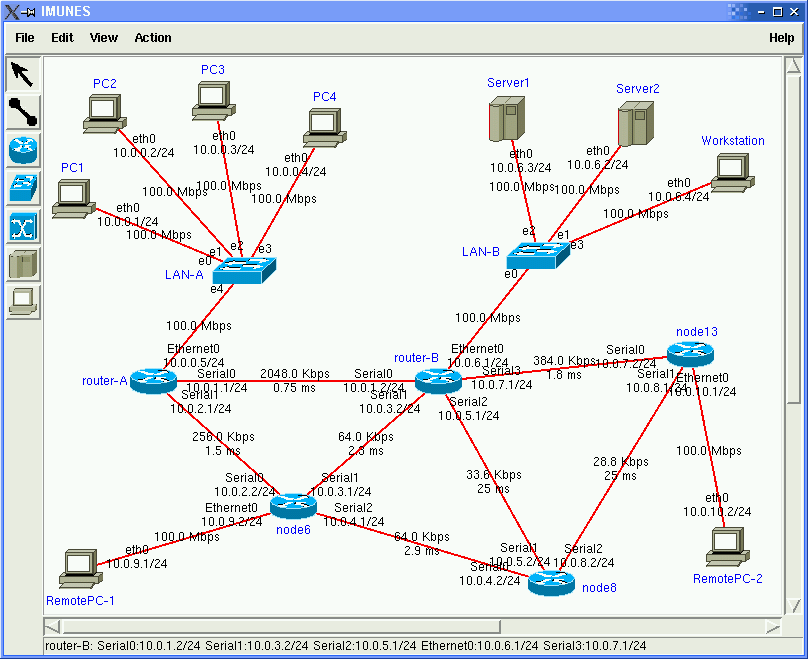
\includegraphics[width=9cm]{images/imunes_gui_normal.png}
	\caption{GUI per il software di emulazione IMUNES.}
	\label{figura:imunes_gui}
\end{figure}

\paragraph{Marionnet}\cite{MVNL08} è anch'esso un ambiente di emulazione di reti virtuali. Permette all'utente di definire, configurare ed istanziare reti di computer anche complesse senza alcun bisogno di apparati fisici. Scritto in \textit{OCaml} ed appogginadosi su \emph{User Mode Linux}\footnote{\emph{User Mode Linux} (UML) da la possibilità di avviare varie \virtualmachine{} con sistema \linux{} (sistema ``Guest'') per eseguire applicazioni come quello che accade con un normale sistema \linux{} (sistema ``Host''). Ogni sistema guest è una normale processo avviato in \emph{user space}.} e \textit{VDE}\footnote{VDE è un  rete virtuale compatibile con ethernet che può essere configurata su una rete di computer fisici su Internet. VDE fa parte del progetto \textit{VirtualSquare}.}, offre una interfaccia grafica molto intuitiva.
\begin{figure}[!ht]
	\centering
	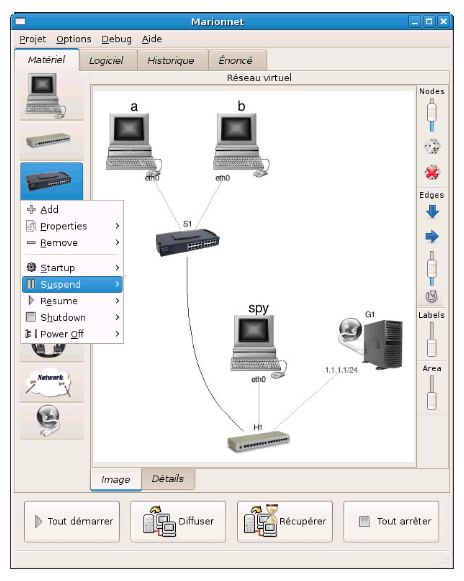
\includegraphics[width=9cm]{images/marionnet_gui.png}
	\caption{Finestra principale di Marionnet mostra una rete composta da tre computer, uno switch un hub ed un gateway.}
	\label{figura:marionnet_gui}
\end{figure}

\netkit{}\cite{NETKIT}  e \emph{VNUML}\cite{VNUMLT} sono entrambi emulatori di medie dimensioni che utilizzano un kernel \emph{User Mode Linux} e permettono di avere importanti esperienze in ambito di reti emulate anche complesse.

\paragraph{Netkit}In \netkit{} una rete viene modellata come la connessione di macchine virtuali. Per la creazione di un lab è necessario creare un file di configurazione per il lab stesso, in cui si descrive la topologia della rete, e alcuni file e directory per ogni virtual machine che si vuole connettere alla rete. In figura \ref{figura:netkit_lab} viene riportato un esempio di struttura di un \netkit{} laboratory.

\begin{figure}[!ht]
	\centering
	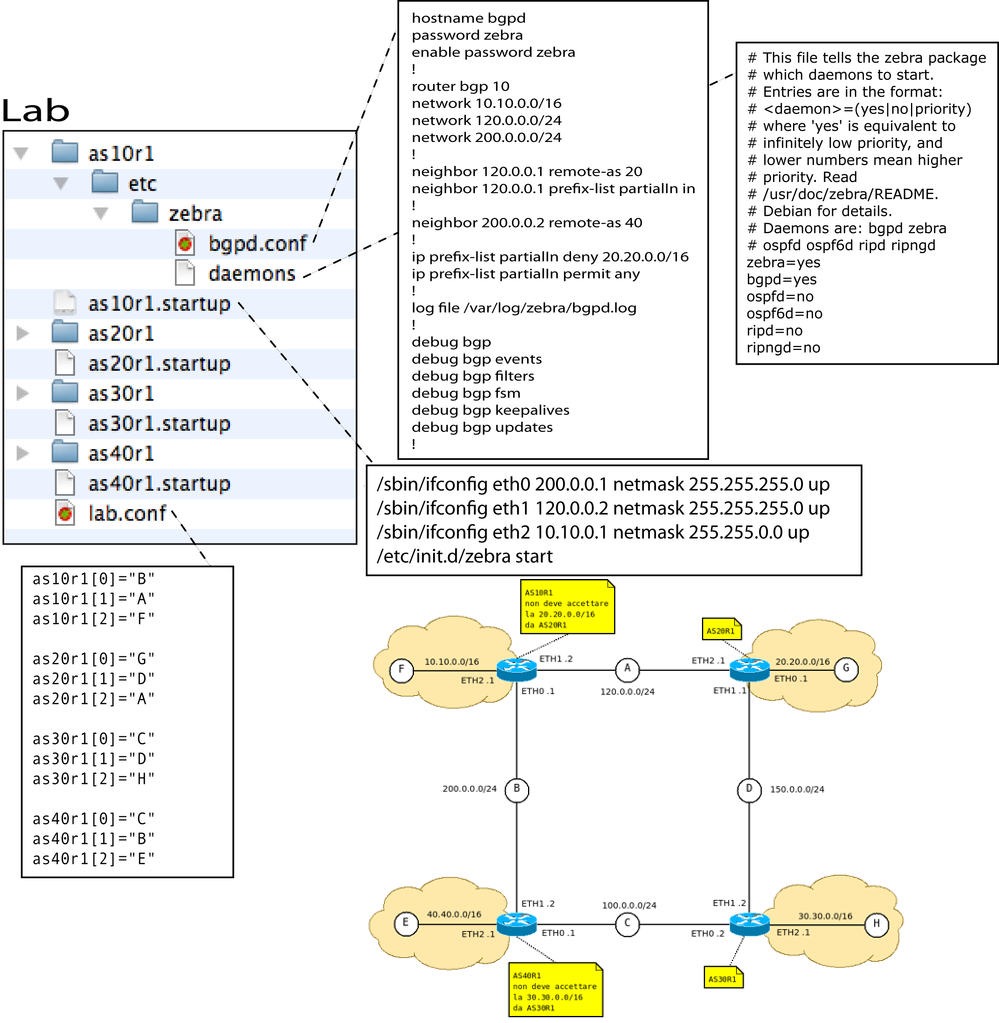
\includegraphics[width=10cm]{images/netkit_lab.png}
	\caption{Schema di rete di un semplice lab in \netkit{} con relativa configurazione.}
	\label{figura:netkit_lab}
\end{figure}

L'interazione tra l'utente finale e le macchine virtuali è possibile per mezzo di una interfaccia a riga di comando tramite terminali emulati (\linux{} shell) un po' come se si stesse davanti an usa sessione \emph{SSH}\footnote{SSH (Secure SHell, shell sicura) è un protocollo che permette di stabilire una sessione remota cifrata ad interfaccia a linea di comando con un altro host.}.


\paragraph{Vnuml}\cite{VNUMLT} (Virtual Network User Mode Linux) è un ambiente di emulazione di reti che raccoglie una serie di script utilizzati per la descrizione di \testbed{} in \xml{}, per il test di applicazioni di rete e servizi.

VNUML consiste in un linguaggio basato su \xml{}, con una specifica sintassi, e di un interprete che può essere utilizzato per descrivere ed eseguire una rete emulata di macchine virtuali UML.
Dalla descrizione in \xml{} degli scenari, VNUML istanzia le macchine virtuali UML e le configura nascondendo all'utente i dettagli avanzati e la configurazione virtuale delle macchine. Questo ambiente risulta molto utile per testare reti anche complesse. Comunque, i progettisti devono descrivere il completo scenario di rete utilizzando il linguaggio \xml{} che, a volte, richiede dettagli molto specifici.

Ad affiancare questo ambiente allo scopo di introdurre una rappresentazione grafica intuitiva è stato realizzato \emph{VNUMLGUI}\cite{VNUMLGUI}. \emph{VNUMLGUI} è un'interfaccia grafica per VNUML.
Esso è soprattutto un editor di topologia con capacità grafiche. Permette di creare qualsiasi topologia di rete virtuale in VNUML senza dover editare manualmente il file \xml{} ma con la sola immissione di router e interruttori.
Così come VNUML nasconde la curva di apprendimento di UML, \emph{VNUMLGUI} nasconde la curva di apprendimento di VNUML e \xml{}.

Di seguito sono riportati a titolo di esempio uno schema di rete e la sua corrispettiva implementazione in VNUML ed una raffigurazione dell'interfaccia grafica di \emph{VNUMLGUI}.

\begin{figure}[!ht]
	\centering
	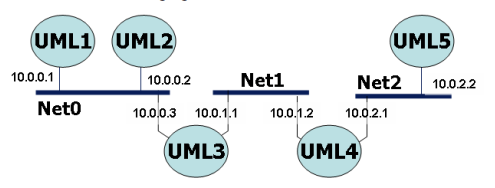
\includegraphics[width=9cm]{images/vnuml_01.png}
	\caption{Schema di rete di un semplice scenario in VNUML con relativa configurazione.}
	\label{figura:vnuml_gui}
\end{figure}

Sia \netkit{} che VNUML sono emulatori realizzati per offrire all'utente una rappresentazione ad alto livello della rete modellata. \emph{NETGUI} e \emph{VNUMLGUI} concretizzano tale scopo. Tutto ciò conferma l'intuizione che è dietro questo progetto e l'importanza di un supporto grafico facile da usare.

\begin{figure}[!ht]
	\centering
	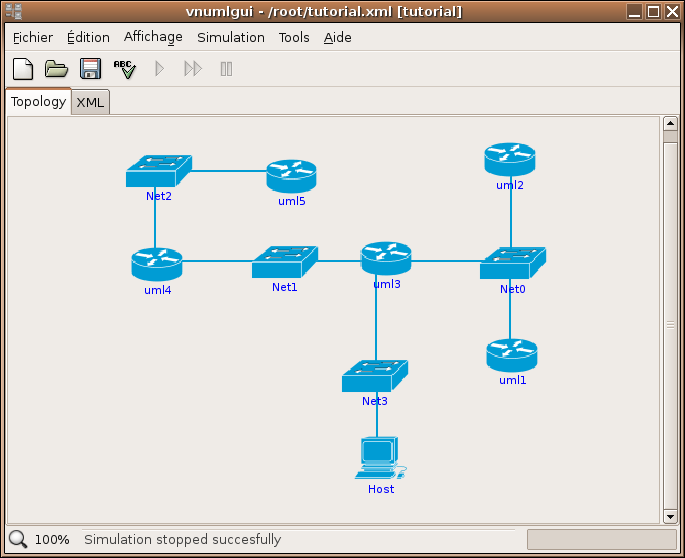
\includegraphics[width=9cm]{images/vnumlgui.png}
	\caption{Schema di rete realizzato in \emph{VNUMLGUI}}
	\label{figura:vnumlgui}
\end{figure}

\paragraph{Qemu}\cite{QUATC05} è un emulatore e virtualizzatore di macchine che fa uso di una traduzione dinamica per ottenere una buona velocità di emulazione. QEMU offre due modalità operative: full system emulation ed user mode emulation, entrambe accessibili tramite interfaccia a riga di comando. Nella prima modalità QEMU emula un sistema completo (ad esempio un PC), tra cui uno o più processori e le varie periferiche. Nella seconda modalità QEMU può avviare processi compilati per una \emph{CPU} su un'altra \emph{CPU}.

QEMU è capace di simulare diverse VLAN\footnote{Il termine VLAN (Virtual LAN) Indica un insieme di tecnologie che permettono di segmentare il dominio di broadcast che si crea in una rete locale (tipicamente IEEE 802.3) basata su switch, in più reti non comunicanti tra loro.}. Una VLAN può essere rappresentata da un collegamento virtuale tra diversi dispositivi di rete quali ad esempio schede Ethernet virtuali QEMU o dispositivi Ethernet su host virtuali.

\section{Ambienti di configurazioni a confronto}
In questa sezione concentreremo gli sforsi sul paragonare le interfaccie grafiche (e quindi gli ``ambienti di configurazione'') che i vari sistemi di \emulazione{} descritti precedentemente mettono a disposizione. Quindi verranno messe a confronto le varie interfacce grafiche di: \emph{Imunes}, \emph{MarionNet}, \emph{VnUMLGUI} e la versione $1.0$ di \visualnetkit{}. In particolare si vuole dare al lettore una panoramica completa su come questi ambienti offrono flessibilità e configuarabilità davanti a configurazioni complesse di reti di calcolatori.

\subsection{Creazione di configurazioni di reti complesse}
Iniziamo con il parlare in \emph{Imunes} e di come sia possibile creare configurazioni complesse\footnote{Per configurazione ``complessa'' si intende una configurazione di un qualche servizio all'intnerno di una \virtualmachine come ad esempio un firewall, un DNS, un server HTTP, un servizio di Routing Interdomain, ecc\ldots}.
Questo ambiente offre una GUI abbastanza semplice scritta in \emph{Tcl/Tk}\footnote{\emph{Tcl} (acronimo di Tool Command Language), è un linguaggio scripting creato da John Ousterhout generalmente considerato di facile apprendimento (rispetto ai linguaggi della sua generazione) ma allo stesso tempo potente. L'estensione \emph{Tk} è un insieme di strumenti per scrivere GUI (un toolkit di widget) implementato dallo stesso autore di \emph{Tcl}.} che offre la possibilità di disegnare una rete a livello topologico inserendo nodi virtuali come Hosts, Switchs e Routers. Tale interfaccia utente è considerata più un front-end verso l'interfaccia a riga di comando che ogni nodo possiede.

Da quanto visto\cite{IMUNESHOWTO}, l'interfaccia grafica che \emph{Imunes} forsisce non offre un adeguato supporto alle configurazioni complesse; in particolare su ogni host occorre effettuare i vari settaggi con il minimo supporto grafico. Viene offerta la possibilità di settare il tipo di Router (Statico o con software \emph{Quagga}) senza però poter settare le varie politiche di routing. Viene inoltre data la possibilità di settare indirizzi IPv4 nei links, rotte statiche nei vari nodi e negli switches è possibile settare parametri quali uso della cpu, politica e dimensione delle code (Queue), ecc\ldots

\emph{MarnionNet} utilizza un'interfaccia grafica ben più potente di \emph{Imunes}. Tramite essa l'utente può disegnare\cite{MVNL08} la topologia di rete desiderata inserendo:
\begin{itemize}
 \item Computers - per ognuno di questi è possibile configurare l'ammontare di memoria RAM e il numero di Ethernets/Serial ports con la possibilità (per le porte Ethernet) di settare indirizzi MAC, IPv4/6, MTU, e nome (figura \ref{figura:marionnet_interfaces});
 \item Hubs e Switches - per ogni hub o switch l'utente può specificare il numero di porte, e (per gli switches) il supporto al protocollo \emph{STP}\footnote{Lo \emph{Spanning Tree Protocol} è un protocollo che previene cicli in una topologia di rete LAN switchata.};
 \item Routers - è possibile inserire routers che usano \emph{Quagga}\footnote{\emph{Quagga} è un derivato del progetto \emph{Zebra} (www.zebra.org) che permette di utilizzare protocolli quali BGP, RIP, OSF e ISIS} come software per il routing statico e dinamico non offrendo però la possibilità di gestire graficamente le varie configurazioni dei servizi e dei protocolli utilizzati;
 \item External Socket e Coulds - \emph{MarionNet} offre anche la possibilità di inserire ``nuvole'' (aggregatori di elementi) con esattamente due endpoints e connessioni verso il sistema Host.
\end{itemize}

Il tutto quindi risulta sviluppato staticamente all'interno del sistema grafico e di conseguenza comporta una rigidità troppo pronunciata per poter essere di effetivo supporto alle configurazioni avanzate dei vari elementi. Basti pensare che ogni servizio all'interno di ogni Host virtuale va configurato senza nessun supporto da parte di \emph{MarionNet}.

\begin{figure}[!ht]
	\centering
	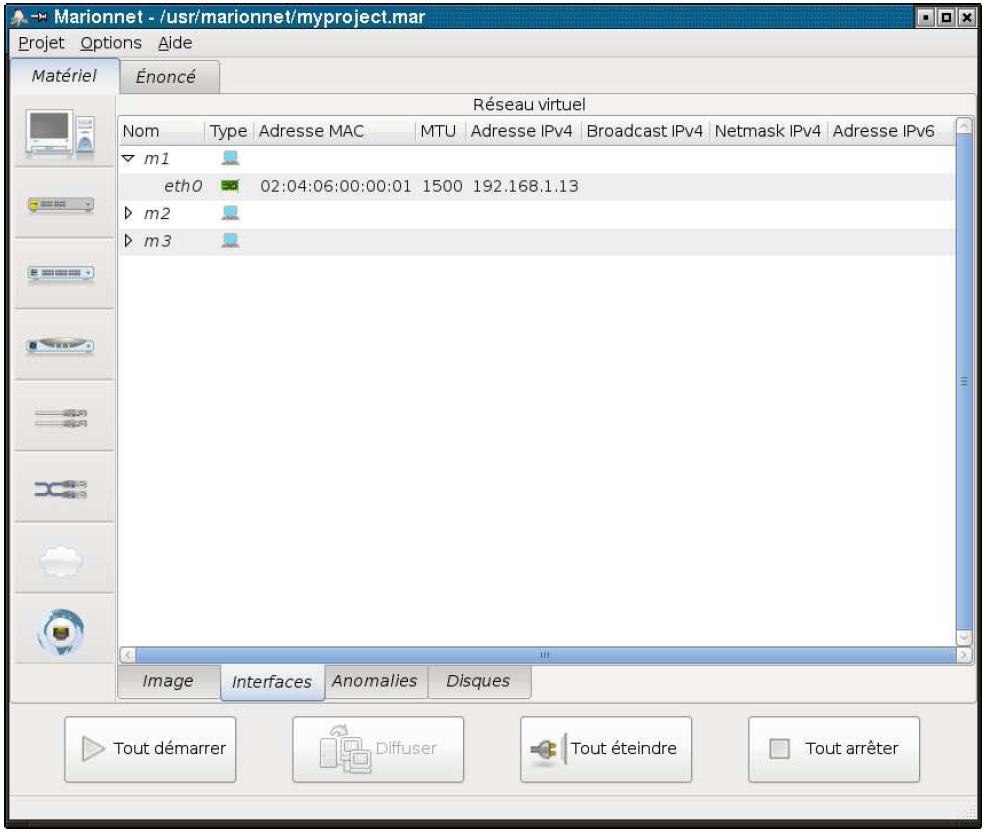
\includegraphics[width=8cm]{images/marionnet_interfaces.png}
	\caption{Setting dei parametri delle interfaccie ethernet in \emph{MarionNet}.}
	\label{figura:marionnet_interfaces}
\end{figure}

Per quanto riguarda \emph{VnUMLGUI} possiamo dire che tale interfaccia utente è la più semplice di quelle sperimentate. Questa offre solamente la possibilità di disegnare la topologia della rete e ricavarne un file \xml che utilizzerà in seguito VNUML per la simulaziene effettiva. Scritto in poche righe di \emph{Perl}, risulta tuttavia un ottimo strumento da affiancare a VNUML, poichè la scrittura della topologia tramite un file \xml è spesso una pratica onerosa e non banale.

\subsubsection{La prima versione di \visualnetkit{}}
È arrivato il momento di parlare di un ambiente grafico per creazione di reti virtuali molto flessibile e innovativo: \visualnetkit{}. \visualnetkit{} è un tool grafico che permette di creare laboratori per \netkit{} disegnando la topologia della rete che si vuole emulare, e allo stesso tempo offre un buon supporto alla configurazione dei vari nodi e archi del grafo. Per nodi e archi in questo caso si intendono da una parte hosts virtuali e ``domini di collisione'', dall'altra links che connettono interfaccie ethernet dei singoli host con uno dei domini di collisione (figura \ref{figura:vn_graph_1}).

\begin{figure}[!ht]
	\centering
	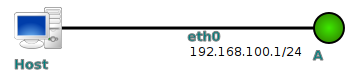
\includegraphics[width=7cm]{images/visualnetkit_graph_1.png}
	\caption{Una semplice rete virtuale in \visualnetkit{}.}
	\label{figura:vn_graph_1}
\end{figure}

Questo tool a differenza degli altri visti precedentemente è stato creato attorno al concetto di flessibilità; infatti \visualnetkit è stato realizzato al di sopra di una struttura a \plugin{} i quali hanno il compito di arricchire la rete a livello di configurazioni e componenti attivi sui vari elementi che costituiscono la topologia del grafo. Questo ambiente (allo stato attuale) non consente di avviare direttamente i laboratory che produce in quanto si è voluto creare un sistema autonomo indipendente da \netkit{} stesso.

Parlando più in dettaglio della sua stuttura modulare, possiamo dapprima osservare che \visualnetkit{} senza alcun \plugin{} attivo offre solamente la possibilità di costruire la topologia della rete virtuale che si vuole sperimentare; è quindi possibile inserire hosts, domini di collisione e links di connessione. Tutto ciò permette a \visualnetkit{} di creare un laboratorio funzionante in tutti i suoi aspetti, ma privo di configurazioni ulteriori.
Per avere una visione più chiara, si osservi la figura \ref{figura:vn_graph_1}. Si può osservare che la topologia è composta da tre elementi base: un host, un dominio di collisione e un link. Soffermandoci su quest'ultimo possiamo notare che vi è un dettaglio che va oltre la semplice topologia di rete; su quel link è stato attivato un \plugin{} di tipo IPv4. Questo quindi permette al link di arricchire il proprio bagaglio informativo aggiungendo in questo caso la possibilità di settare ulteriori paramentri (propriamente contenuti all'interno dei plugins) quali \emph{address}, \emph{netmask} e \emph{broadcast}. Chiaramente queste informazioni aggiuntive dovranno essere salvate all'interno del laboratorio che si sta creando; in questo caso il sistema prevede che ogni \plugin{} possa fornire un numero arbitrario di ``contributi'', ossia porzioni di file di testo (e relativo percorso del file interessato) che costituiranno il file di configurazione per quel determinato plugin. In figura \ref{figura:vn_graph_2} è possibile osservare come il \plugin{} IPv4 attivo sul link sia il diretto responsabile del contenuto del file di configurazione della macchina ``Host''.

\begin{figure}[!ht]
	\centering
	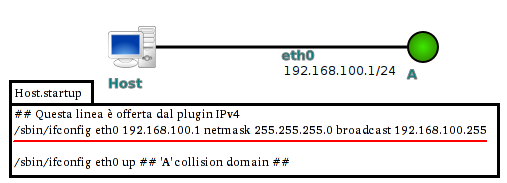
\includegraphics[width=9cm]{images/visualnetkit_graph_2.png}
	\caption{Relativo file di configurazione della rete in figura \ref{figura:vn_graph_1}.}
	\label{figura:vn_graph_2}
\end{figure}

Come detto ogni \plugin{} offre informazioni agguntive all'elemento base a cui è stato collegato; scendendo un po' nel dettaglio possiamo dire che i vari \plugin{} possono offrire un insieme di proprietà descritte da una lista di coppie chiave-valore. Nel nostro esempio, il plugin IPv4 offre una lista di tre ``property'':
\begin{itemize}
	\item \textbf{address} - l'indirizzo ipv4;
	\item \textbf{netmask} - la netmask associata;
	\item \textbf{broadcast} - l'indirizzo broadcast.
\end{itemize}

Queste proprietà sono comunque statiche all'interno dei vari \plugin{} e l'utente può solamente limitarsi a modificarle previo controllo di errori non vincolante. Abbiamo quindi trovato uno dei punti deboli che la priva versione di \visualnetkit{} possiede; anche se basata su una struttura modulare e flessibile, i plugin stessi limitano tale flessibilità rimanendo troppo rigidi per offrire un buon supporto in situazioni dove sono necessarie configurazioni avanzate.

Abbiamo appena anticipato un problema che durante il seguente lavoro tratteremo più in dettaglio, mostrando come la nuova versione del tool grafico offra maggior flessibilità e risolva in gran parte il problema appena accennato. In figura \ref{figura:vn_main_1} viene mostrato l'ambiente grafico offerto da \visualnetkit{} versione $1.0$.

\begin{figure}[!ht]
	\centering
	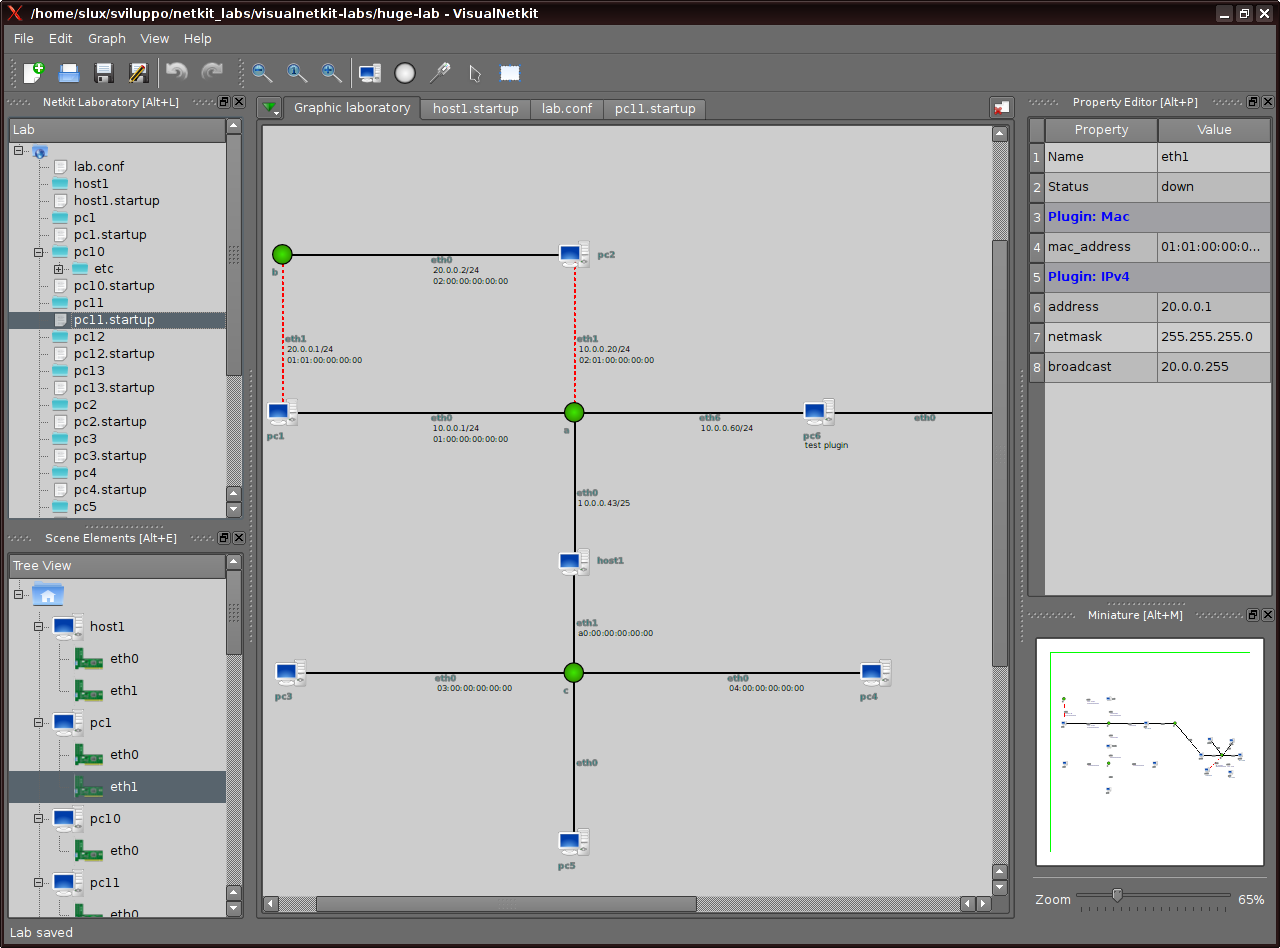
\includegraphics[width=12cm]{images/visualnetkit_main_1.png}
	\caption{Un laboratorio creato con \visualnetkit{} versione $1.0$.}
	\label{figura:vn_main_1}
\end{figure}

\subsubsection{Flessibilità delle interfaccie grafiche nei sistemi esistenti}
Abbiamo appena visto come l'avere un ambiente grafico di supporto sia altrettanto imporntante del supporto offerto dal sistema di \emulazione{} stesso. Avere infatti uno strumento potente per creare i nostri laboratori, ma che possegga specifiche di creaziene complicate e poco intuitive, può indurre l'utente ad evitare di addentrarsi in particolari configurazioni avanzate poiché vi è un forte rischio di dispendio di energie e di un elevato tempo di creazione.
È in questo preciso istante che entrano in gioco i tools grafici pocanzi descritti.

Riassumendo possiamo affermare che tra le interfaccie grafiche viste fin'ora, nessuna riesce ad offrire un supporto totale; ognuna infatti prevede una parte di configurazione manuale ossia, l'utente che vuole addentrarsi in configurazioni particolari, deve necessariamente agire direttamente sui vari file di configurazione dei vari nodi della rete, o in alcuni casi deve intervenire interattivamente tramite le interfaccie a riga di comando previste per ogni \virtualmachine. \\
Di seguito (tabella \ref{figura:gui_compare}) viene proposta una tabella riassuntiva che paragona i vari strumenti.

\begin{figure}[!htb]
	\centering
	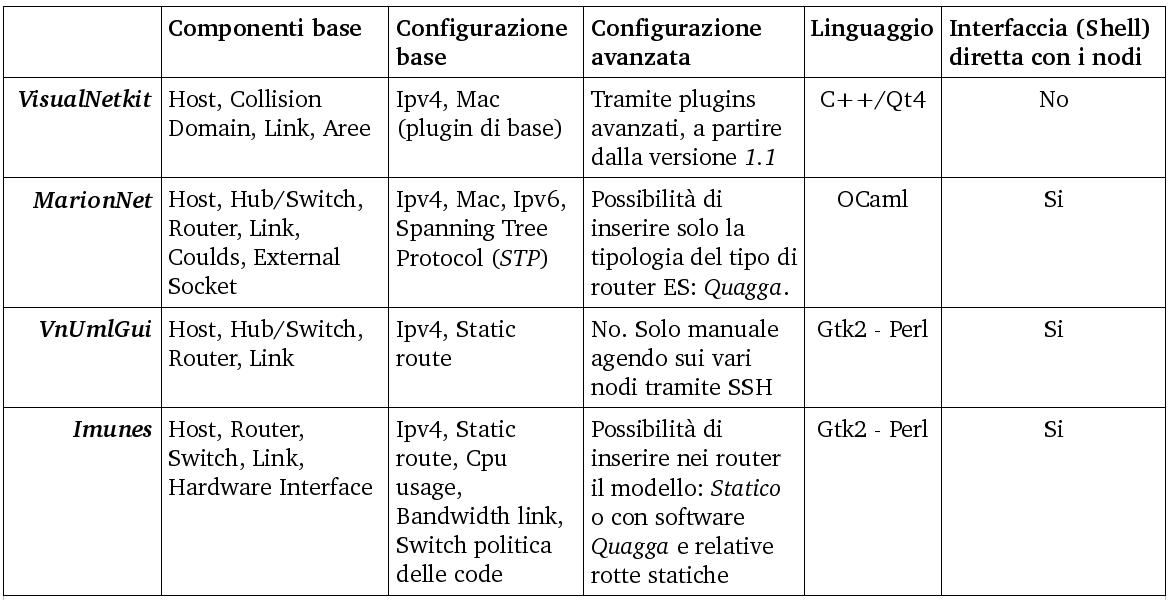
\includegraphics[width=12.7cm]{images/tabella_comparativa.png}
	\caption{Tabella comparativa delle interfacce grafiche analizzate.}
	\label{figura:gui_compare}
	
\end{figure}
